\subsection{RDF Vocabulary}

A mechanism for decentralized description and discovery of data we proposed
over two decades ago \textcolor{red}{cite https://www.w3.org/Talks/WWW94Tim/} 
and exists now in the tools and technologies of the Semantic Web. Especially, 
the specification of RDF as a data interchange format for the World Wide 
Web. \textcolor{red}{cite https://www.w3.org/RDF/?}. Decoupling publication 
from access meets many of our identified requirements (1, 4 and 5) and 
using RDF to describe log data collections provides decentralization 
and discovery without requiring a priori knowledge of other collection 
efforts.

In RDF \emph{things} (concepts or concrete items) are represented as URIs
and arranged in \emph{triples} of a subject, a predicate and an object.  

\begin{figure*}
\begin{minted}{turtle}
@prefix nersc: <http://portal.nersc.gov/project/mpccc/sleak/nersc#> .
@prefix rdfs: <http://www.w3.org/2000/01/rdf-schema#> .
@prefix foaf: <http://xmlns.com/foaf/0.1/> .
nersc:nersc rdfs:type foaf:Organization .
\end{minted}

\caption{A triple of (subject, predicate, object) describes an edge 
in an RDF graph. The \texttt{Turtle}\textcolor{red}{cite} syntax shown
here aids human readability by condensing URIs into a prefix and a suffix,
so for example \texttt{rdfs:type} expands as
\texttt{<http://www.w3.org/2000/01/rdf-schema\#type>}.}
\label{f:rdftriples}
\end{figure*}

For example, we wish to state that NERSC is an Organization. We have a 
\emph{subject} (NERSC), a \emph{predicate} (``is an'') and an \emph{object} 
(Organization). In a manner of pulling oneself up by one's bootstraps, the 
W3C \textcolor{red}{cite https://www.w3.org/} publishes some standard 
vocabularies in the form of URIs that have a well-defined and documented 
meaning, including that \texttt{<http://www.w3.org/2000/01/rdf-schema\#type>}
refers to the predicate ``is a''. Another vocabulary, known as the 
Friend-of-a-friend vocabularies, associates \texttt{<http://xmlns.com/foaf/0.1/Organization>} with the concept of an 
organization. In this spirit we write the triple in Figure~\ref{f:rdftriples}
by associating a URI we've chosen: \texttt{<http://portal.nersc.gov/project/mpccc/sleak/nersc\#nersc>} with the 
organization we know as ``NERSC''. 

A single triple tells us very little, but a collection of many triples 
forms a graph representing almost arbitrary knowledge graph. We get 
decentralization by the use of URIs as graph elements - any contributer 
can publish a set of triples and, so long as \emph{somebody} is aware of 
it, it can be incorporated into a global graph.

The other Semantic Web element key to our requirements is the SPARQL 
graph query language. A SPARQL query 
arranges variables into a set of triples and returns nodes for which
the triples form a true statement. For example, the following SPARQL query
will return the name and interest for each node whose type is 
a subclass of \texttt{foaf:Agent}. \texttt{foaf:Agent} is a superclass for a Person, a 
Group or an Organization, so this query in English is ``list the name and 
interest for each Person, Group or Organization in this graph''. (The 
\texttt{rdfs:subClassOf*} syntax indicates that the query should follow 
\texttt{rdfs:subClassOf} edges to any depth until a \texttt{foaf:Agent} 
is encountered).

\begin{figure}[H]
\begin{minted}{sparql}
SELECT ?name ?interest 
WHERE {    
    ?type rdfs:subClassOf* foaf:Agent .
    ?uri rdfs:type ?type .
    ?uri foaf:name ?name .
    ?uri foaf:interest ?interest .
}
\end{minted}
\caption{Example of a SPARQL query}
\label{f:sparql}
\end{figure}

Figure~\ref{f:sparql-diagram} illustrates how this query might act on a graph: 
the first statement locates nodes from which one can traverse \texttt{rdfs:subClassOf} properties and reach a \texttt{foaf:Agent} - colored blue. The second statement 
locates nodes in triples with an \texttt{rdfs:type} predicate whose object 
is one found by the first statement - shown here in red. Thus far we have found Jim, 
Ann, Annette and Steve. Next we look for triples whose subject is one of those nodes
and whose predicate is \texttt{foaf:name}, reducing the set to Jim, Ann and Steve, then
again for predicate \texttt{foaf:interest}. Now only Steve matches all of the criteria.
Finally, we return the nodes associated with the \texttt{name} and \texttt{interest} 
variables, which in this case are the purple-colored objects of those triples.

\begin{figure}
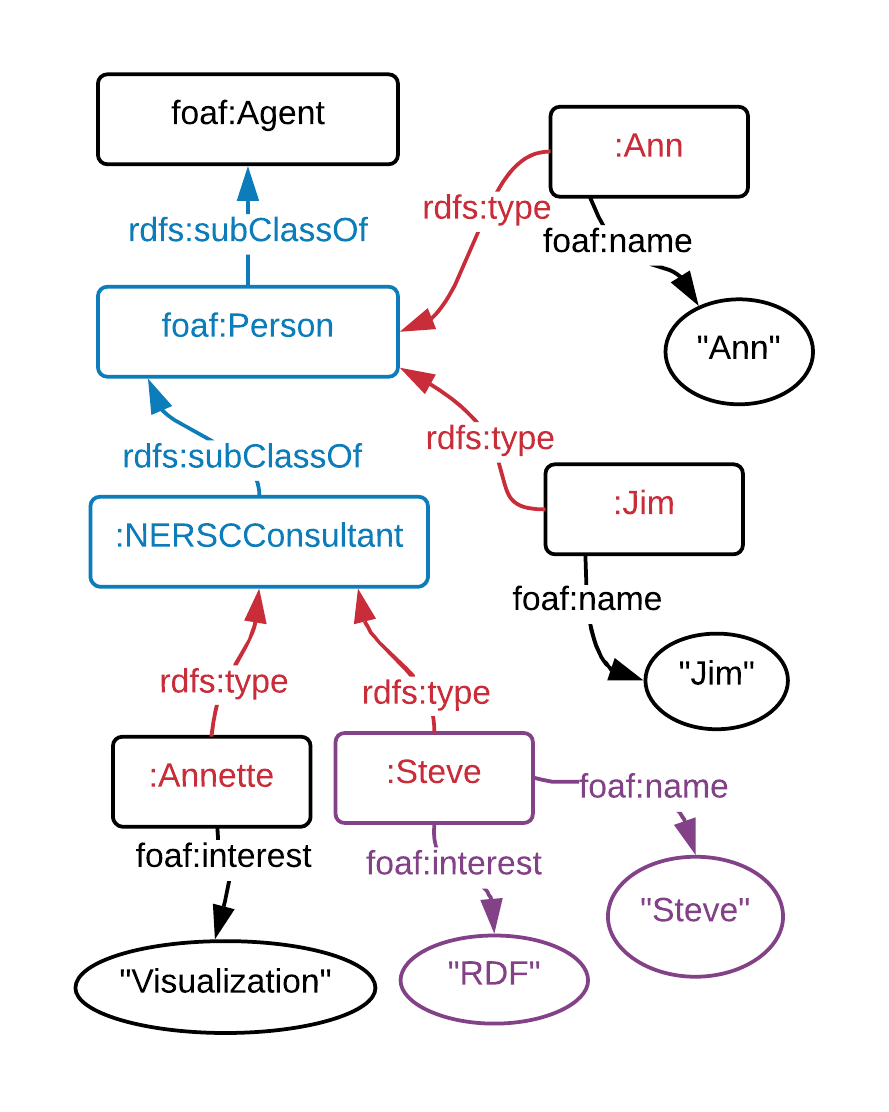
\includegraphics[width=0.4\textwidth]{sparql.png}
\caption{Illustration of the SPARQL query in Figure~\ref{f:sparql} }
\label{f:sparql-diagram}
\end{figure}

\textcolor{red}{TODO: might need a ref to an "intro to semantic web" resource}


\subsubsection{The vocabulary}

The key classes and predicates forming our vocabulary are illustrated in 
Figure~\ref{f:logset-classes}. Figure~\ref{f:logset-classes-nodes} provides 
examples of nodes in a graph corresponding to each class, and an 
illustration of how RDF descriptions of different \texttt{LogSet}s published 
in different places form a single, global graph is show in 
Figure~\ref{f:logset-example}. Particularly, Figure~\ref{f:logset-example}
shows how the vocabulary can be used to publish data dictionaries 
describing different \texttt{SubjectType}s and \texttt{LogSeries}.

The vocabulary is extended and specialized 
from the Data Catalog Vocabulary \textcolor{red}{cite}. The meaning, 
reason and usage of each are as follows:

\begin{description}
\item[Catalog] \hfill

The \texttt{dcat:Catalog} class is used as an access point to LogSet datasets and 
to link disparate collections into a single graph. Catalogs are anticipated to be 
published at a site granularity: staff at a site would publish LogSets under
a URL that the staff member can access, linked to the global graph via a single 
entry in the site Catalog. (The mechanism for this can be as simple as a pull
request to a Github repository).

\texttt{Catalog}s can use \texttt{rdfs:seeAlso} properties to link to other 
catalogs and to data dictionary

\item[LogSet] \hfill

A collection of logs related in system and access and timespan,
for example the logs collected in a \texttt{p0-} directory in the SMW of a Cray
XC for a single boot session. The \texttt{LogSet} should provide a description
of the data and contact information and is an entry point to metadata for 
the \texttt{ConcreteLog}s.

Note that the \texttt{LogSet} itself doesn't necessarily have properties for 
temporal or subject information. We anticipate that these would be derived 
from the \texttt{ConcreteLog}s comprising the \texttt{LogSet}.

A \texttt{LogSet} might be a closed archive or might be ``open'', that is' 
acquiring new logs over time. This is indicated via the \texttt{isClosed} 
property, ..

\item[ConcreteLog] \hfill

A \texttt{ConcreteLog} describes a specific, concrete source of log entries.
This might be a log file but could also be, for example, a Slurm instance
from which job data can be obtained. 

The \texttt{accessURL} and \texttt{downloadURL} have subtly different uses,
inherited from \texttt{dcat:Distribution}. The actual data described by the 
\texttt{ConcreteLog} may not be directly accessible (due to security or 
other practical constraints), in which case an \texttt{accessURL} which 
can help a user to learn about gaining access is more suitable than a 
\texttt{downloadURL}, which is expected to provide direct access to the 
data.


The \texttt{ConcreteLog} also supports a number of properties about the
size, number of records and timespan of the data. For many data sources 
an ill-considered query might result in an excessive volume of data returned,
so these properties are intended to help users check 


\item[LogSeries] \hfill

The console log for a server is often distributed over multiple files,
and is fundamentally the same for servers of the same make at different
sites. A \texttt{LogSeries} allows the common metadata to be published
once in a common dictionary...


\item[LogFormatType]

One level more general than a \texttt{LogSeries}, a \texttt{LogFormatType}
is common to many \texttt{LogSeries}. As an example, many \texttt{LogSeries}
have the form of a \texttt{timeStampedLogFile}. Another significant 
\texttt{LogFormatType} is \texttt{sqlite3DB} (which encapsulates our 
reference implementation of the Annotation Schema~\textcolor{red}{cross-ref})

\item[Subject]
...
affects and partOf



\item[SubjectType]

Each \texttt{ConcreteLog} has a specific \texttt{Subject} - e.g. a 
\texttt{cori} or \texttt{cori\_nid00123}. It is useful to classify 
\texttt{Subject}s by their type so that for example, a researcher 
seeking HSN data can find \texttt{ConcreteLog}s about the HSN 
component of multiple clusters by querying for \texttt{ConcreteLogs}
whose \texttt{subject} is a specific \texttt{subjectType}. 

This also supports cataloging new datasets: rather than asking the
user the \texttt{subject} of each \texttt{ConcreteLog}, we can 

skos:broader, also aspectof


\end{description}

-- some key things to call out:
\begin{itemize}
\item someone publishing a logset doesn't need to know many people to get their 
      logset into the graph - a curator of their local (site) catalog is enough. 
      That curator then knows curators of at least one other catalog and thus 
      gets the local 
      subgraph into the global graph
\item someone using the graph doesn't need to know who published what - they can
      query the graph itself and get metadata about what is out there, including contact 
      information for data they don't directly have access to. This allows them to 
      solve specific access limitations in a locally-appropriate way
\end{itemize}

\begin{figure*}
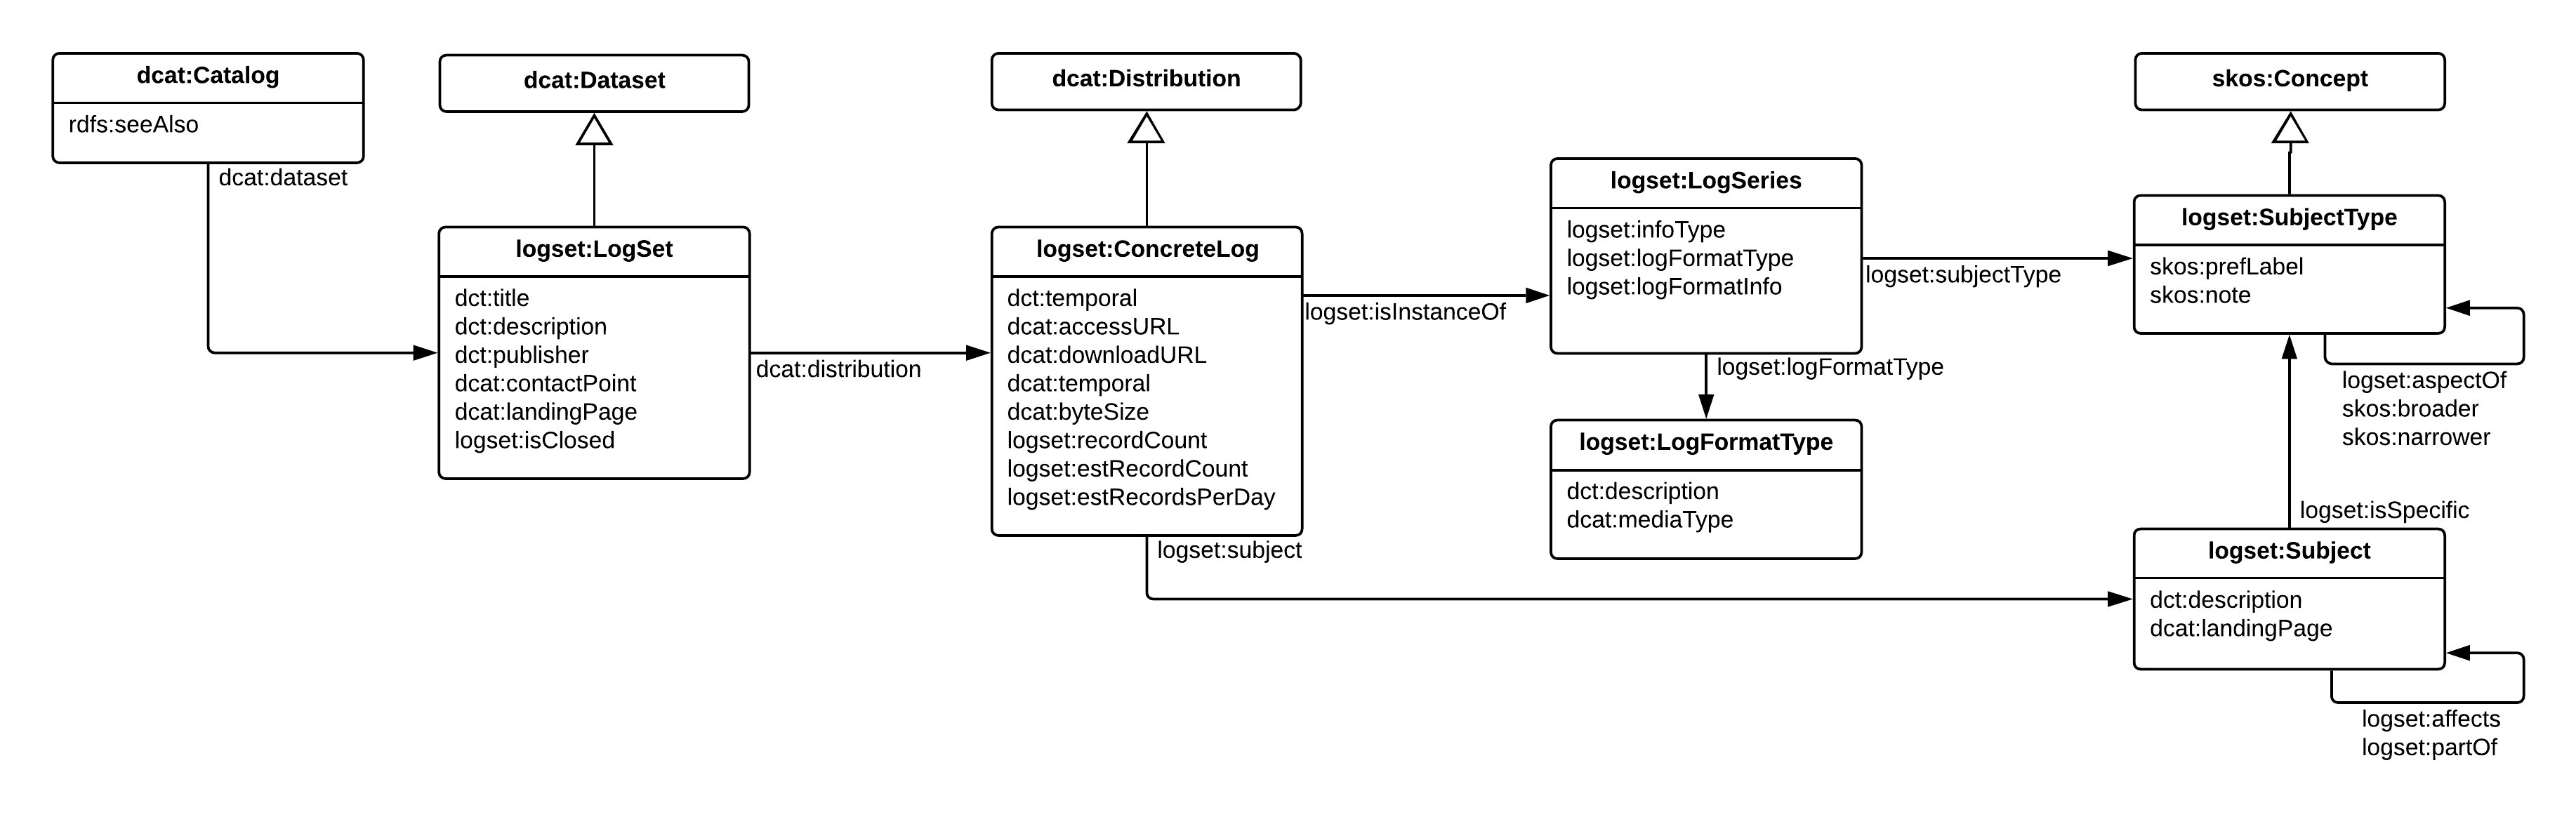
\includegraphics[width=1.0\textwidth]{logset-key-classes.png}
\caption{Key classes and predicates in the logset vocabulary. }
\label{f:logset-classes}
\end{figure*}

\begin{figure*}
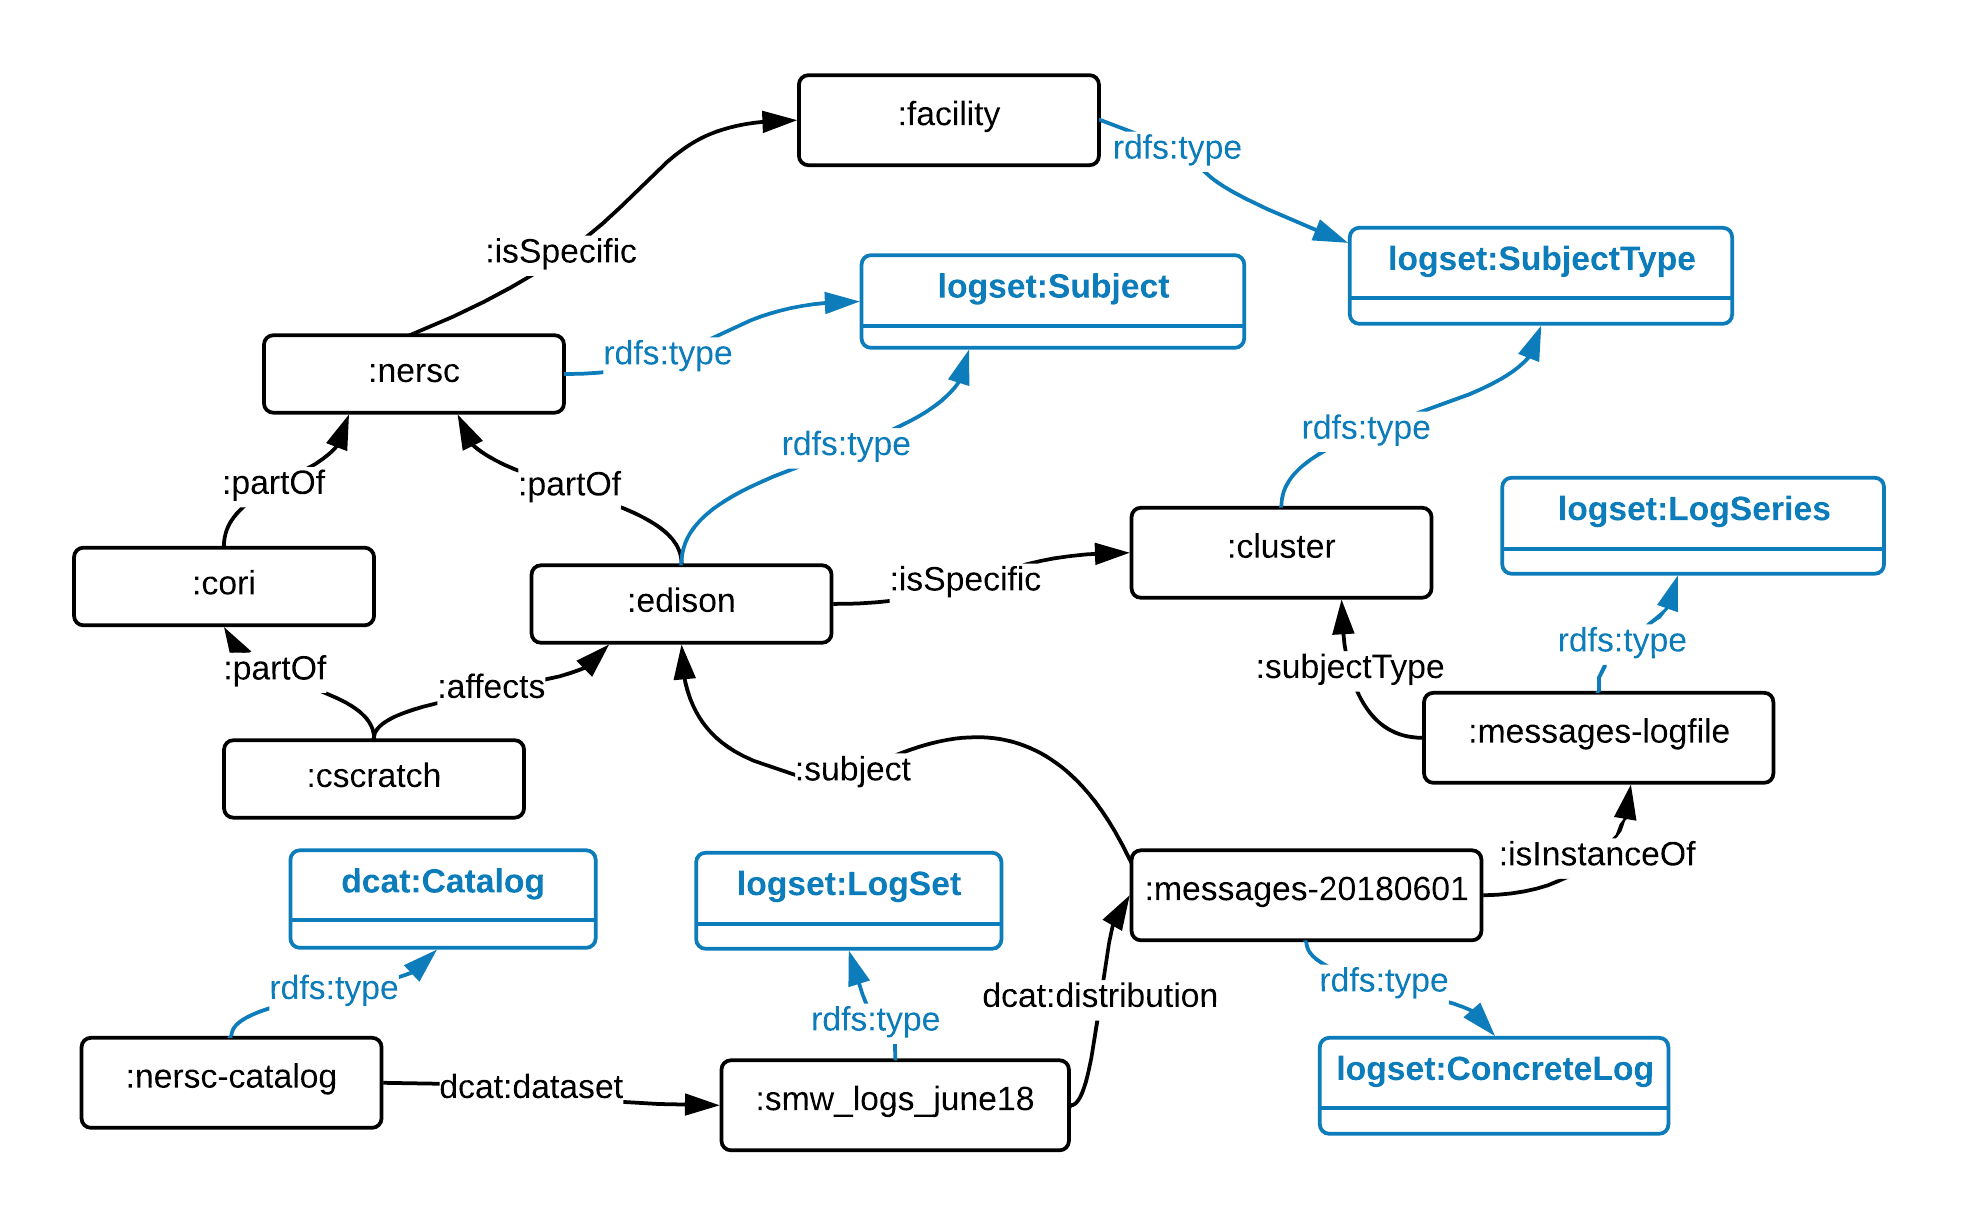
\includegraphics[width=0.9\textwidth]{logset-classes-nodes.png}
\caption{Examples of some nodes and relationships published in different places 
from different sites (indicated via color), forming a single global graph. }
\label{f:logset-classes-nodes}
\end{figure*}

\begin{figure*}
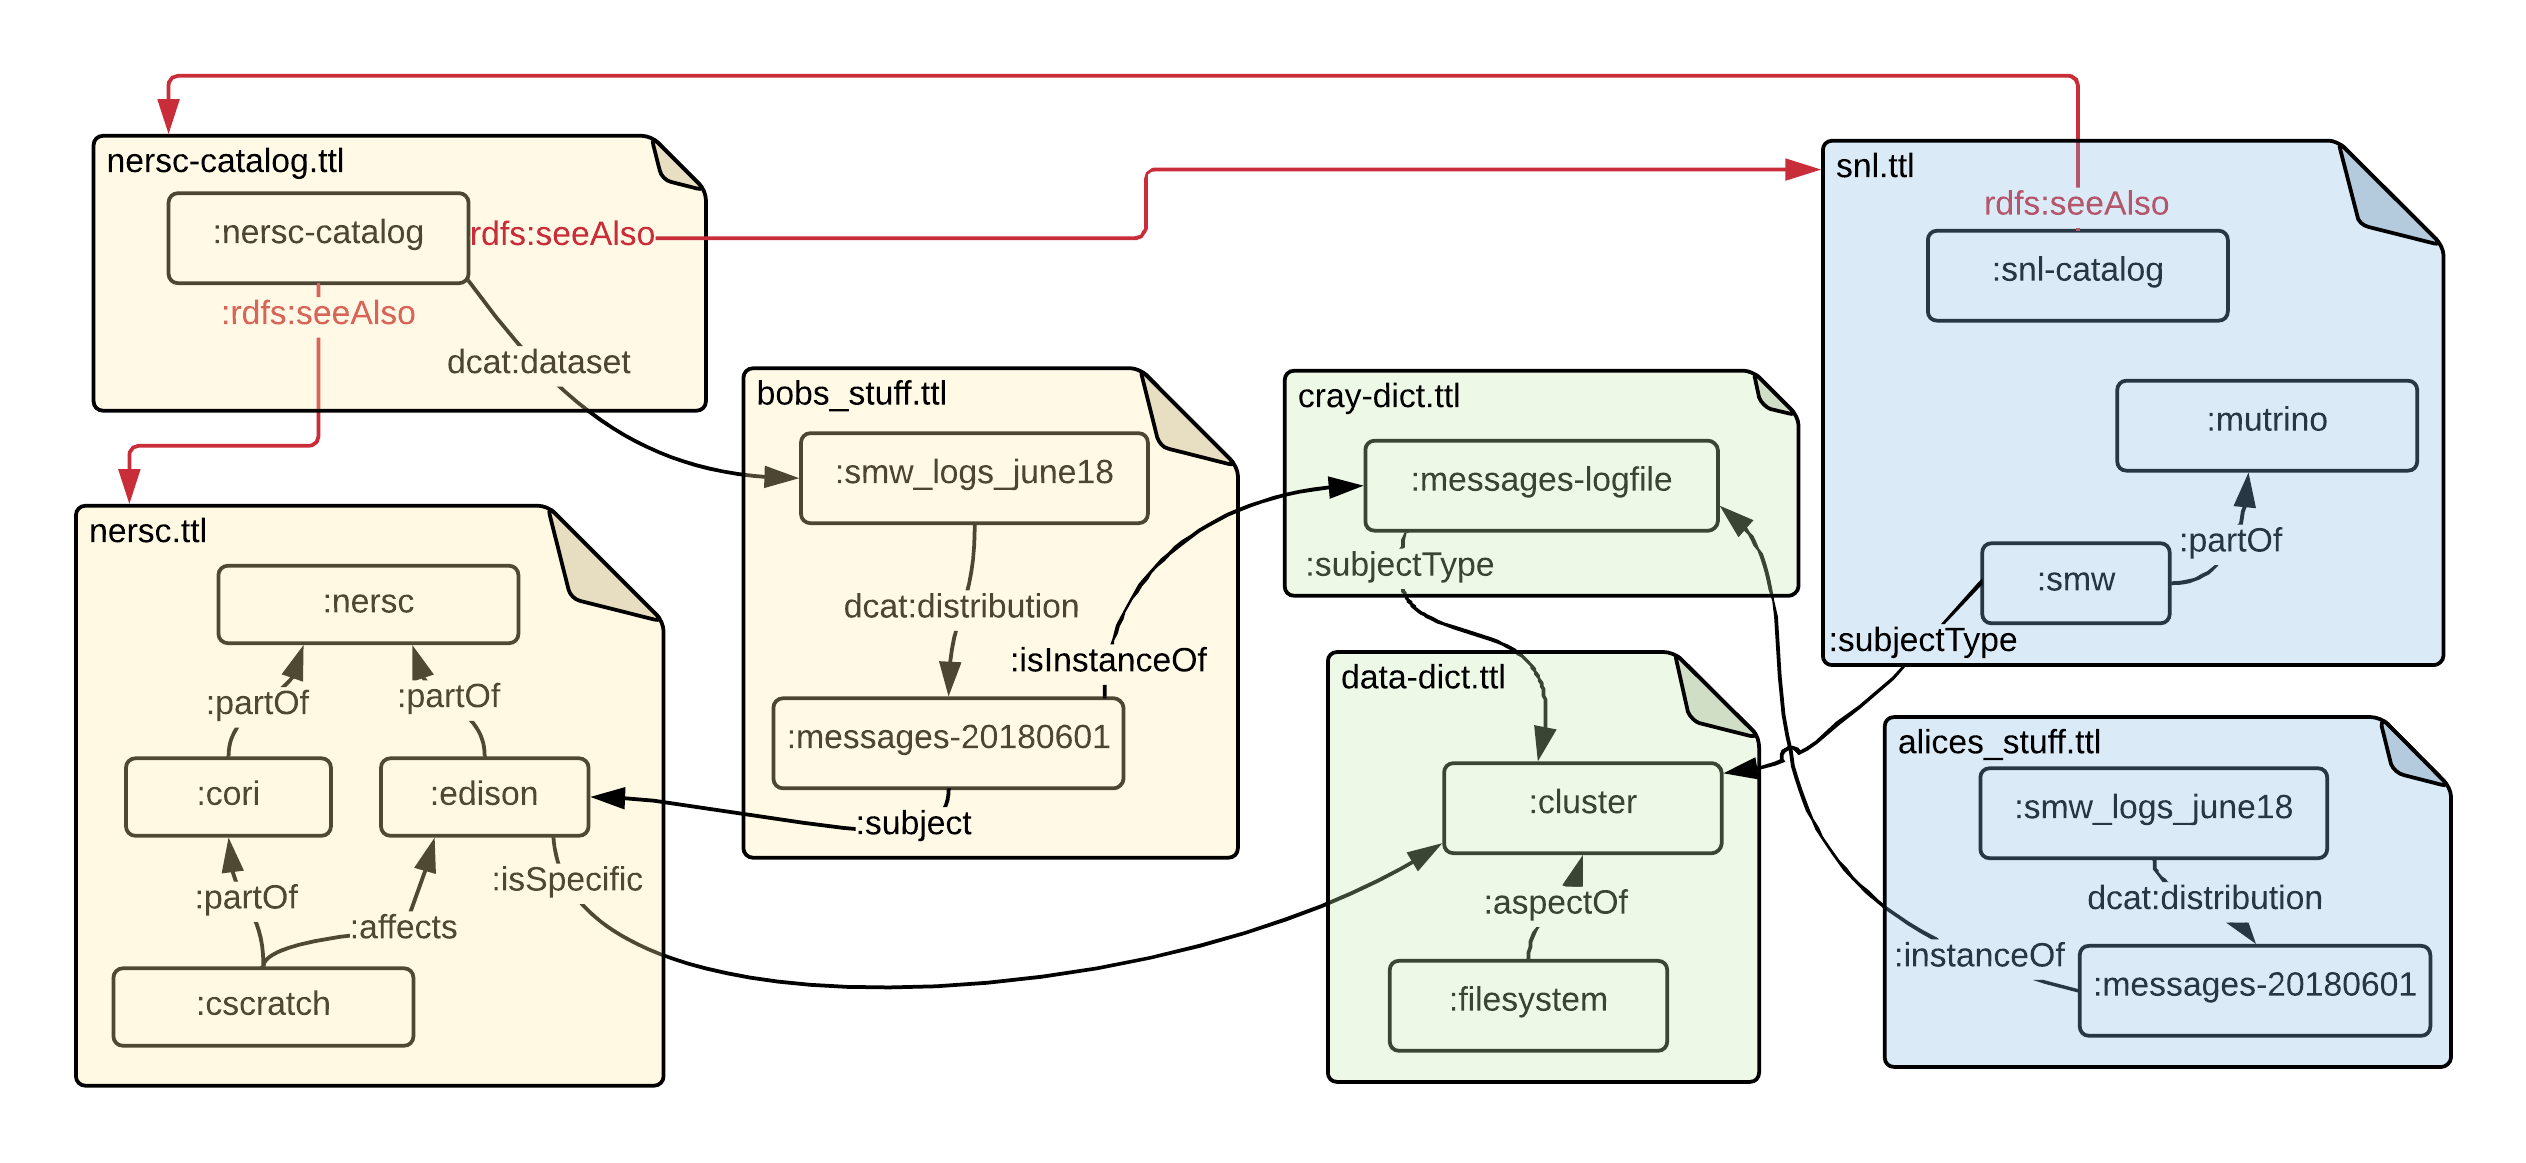
\includegraphics[width=0.9\textwidth]{logset-example.png}
\caption{Key classes and predicates in the logset vocabulary. }
\label{f:logset-example}
\end{figure*}
